\chapter{Comparing the Tree Edit Distance and the generalized Robinson Foulds Distance}
In this chapter we compare the results of our computations. The focus of this work was to find a possibility to resemble the gRF, which is quite time consuming, with a special case of the TED. We start by discussing the time complexity of both measures. Afterwards we discuss the differences between the distances themselves. We take a look whether we can simulate or improve the gRF by considering the TED with a certain distance function.

\section{Time Complexity}
We already talked about the time complexity of each distance measure a little bit in the previous two chapters. Our observations reflect the expected behaviour. Computing the TED was possible for trees with up to about $256$ leaves each in a manageable time of approximately $520$ seconds. The time is pretty much the same for any of the investigated distance measures. This was roughly the same time as it took to find the gRF of trees with $24$ leaves each.
\begin{figure}[!ht]
	\centering
	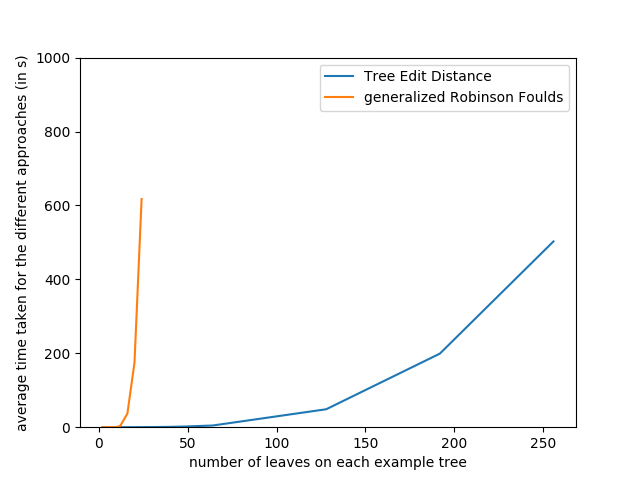
\includegraphics[width=0.6\textwidth]{figures/time_plot_all.png}
	\caption{This graph shows the time it took to compute the distance measures between two trees with up to $256$ leaves.}
	\label{fig:time}
\end{figure} 
The graph shows, that as soon as the examples reach a size of about $20$ leaves each, the time to compute the gRF distance explodes. Depending on the computational possibilities, it might not be possible to compute real life instance where the trees have $50$ leaves. On the other hand the time to compute larger instances of the tree edit distance remains manageable even for bis instances. The curve looks very much like a polynomial curve, just as we expected.

\section{Discussing the Results}
For the comparison of the gRF with the TED, we will concentrate on a single TED. In the previous chapter, we discussed that the CTED is mainly concentrating on the permutation of the leaves' labels, not on the structure of the trees. On the other hand, the STED is not representative, as the costs are very much dependent on changes among the interior nodes, whereas they don't impact the gRF directly. Thus we will use a compromise of the similarities of the gRF with the STED and the CTED respectively, namely the $\frac{1}{2}$-ATED. \\
To be able to compare the $\frac{1}{2}$-ATED and the gRF we concentrated on trees with $20$ leaves each. This number is a compromise between the performance to compute the gRF and a big size of the test instances. In this way we were able to compute $300$ test instances.

We know, that the $\frac{1}{2}$-ATED is much easier to compute than the gRF for a given instance. Thus we would very much benefit if it would be possible to use the $\frac{1}{2}$-ATED to "simulate" the gRF. To get a feeling whether or not this is possible, we may ask the following questions:
\begin{enumerate}
	\item Does a low gRF imply a low $\frac{1}{2}$-ATED?
	\item Does a low gRF require a low $\frac{1}{2}$-ATED?
	\item Does a high gRF imply a high $\frac{1}{2}$-ATED?
	\item Does a high gRF require a high $\frac{1}{2}$-ATED?
\end{enumerate}
Before we answer these questions, let's take a look at two unpromising examples:

\textit{Example low gRF, high $\frac{1}{2}$-ATED}:\\
The first example is illustrated in Figure~\ref{fig:lght}, it was also used in the previous chapter. It is obvious, that the trees $T_1$ and $T_2$ have the same clusters, therefore the gRF has to be $0$. But since the order of the leaves' labels is reversed, the shortest $\frac{1}{2}$-ATED is $8$ and can be obtained by relabelling all leaves. 
\begin{figure}[!ht]
	\centering
	\caption{Two trees $T_1$ and $T_2$ which have a low gRF but a high $\frac{1}{2}$-ATED.}
	\label{fig:lght}
\end{figure} 

\textit{Example low $\frac{1}{2}$-ATED, high gRF}:\\
The second example is illustrated in Figure~\ref{fig:lthg}. The value of the $\frac{1}{2}$-ATED amounts to $4.5$ which can be obtained by $5$ deletions and $4$ insertions. On the other hand, the gRF adds up to $8$. This is the highest gRF between two trees with just $8$ leaves we were able to construct. Furthermore, there hasn't been a randomly generated pair of trees that has a similar gRF distance. On the same time, the $\frac{1}{2}$-ATED is a quite small distance.
\begin{figure}[!ht]
	\centering
	\caption{Two trees $T_1$ and $T_2$ which have a low gRF but a high $\frac{1}{2}$-ATED.}
	\label{fig:lthg}
\end{figure} 

These two examples shall give an insight into the problems with comparing the $\frac{1}{2}$-ATED with the gRF. They show that it is possible to construct examples, that negate any similarity between the gRF and the $\frac{1}{2}$-ATED. 

\begin{figure}[!ht]
	\centering	
	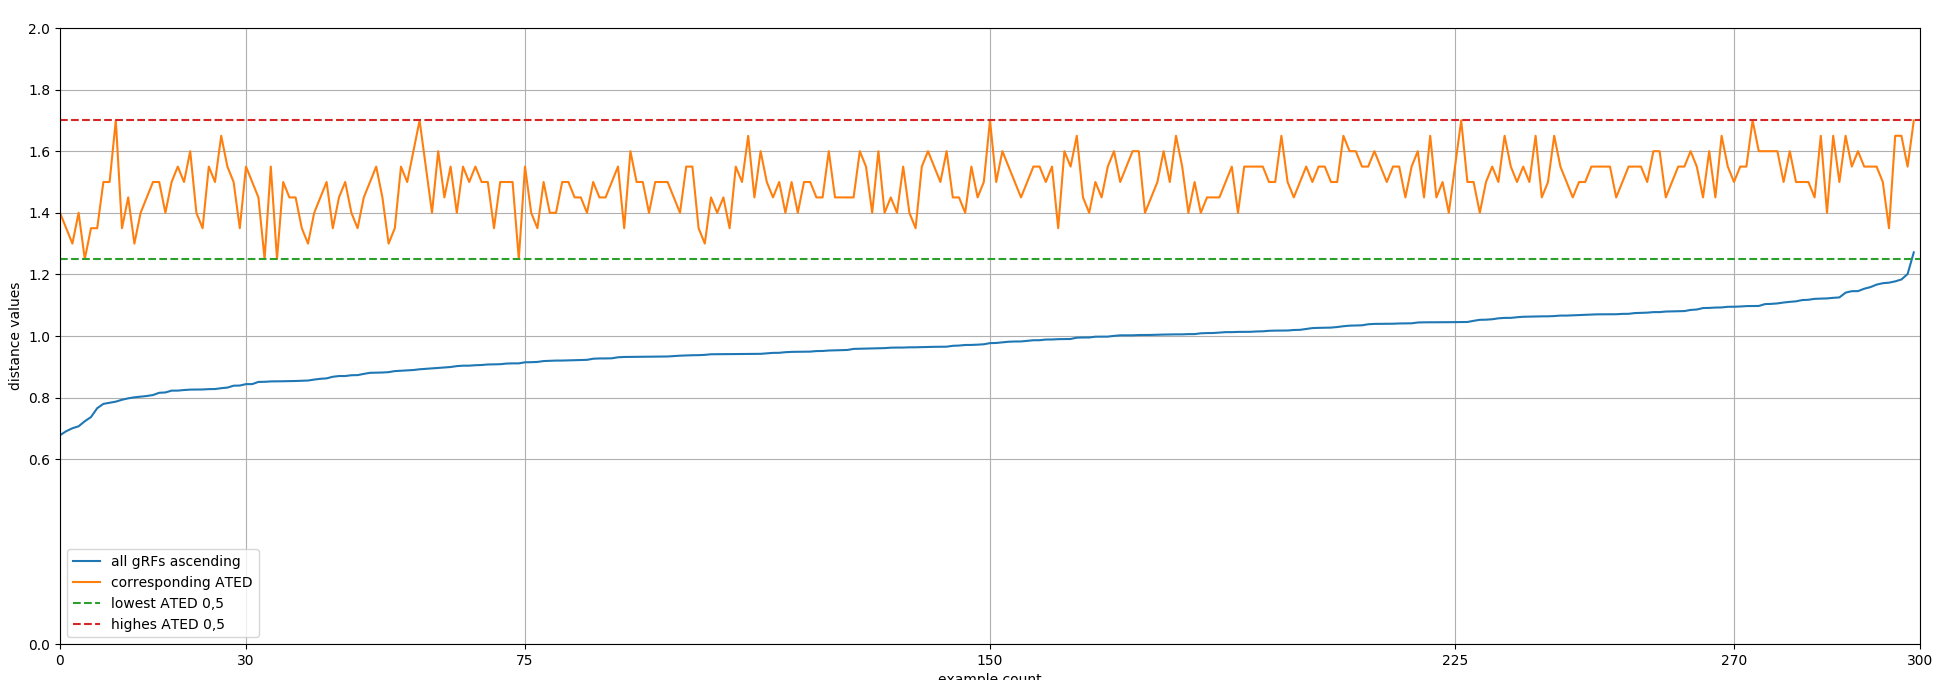
\includegraphics[width=\textwidth]{figures/all_examples_grf_corr_ated.png}
	\caption{Illustration of the distances of our randomly generated test instances, sorted increasingly with respect to the gRF distance.}
	\label{fig:ex_grf_ated}
\end{figure} 
Let's take a look at the results we got from our simulations. Our database consists of $300$ pairs of randomly generated phylogenetic trees with $20$ leaves. We illustrate the distances in Figure~\ref{fig:ex_grf_ated}. Every integer value on the X axis corresponds to an example pairing. Furthermore we sorted the example according to their gRF distance. Therefore the example where $x=1$ has the lowest and the one where $x=300$ has the gRF distance among all example. 

We inserted grid lines at the $10$\%-, $25$\%-, $50$\%-, $75$\%- and $90$\%-marks of the gRF values. Furthermore we marked the highest and the lowest values of all $\frac{1}{2}$-ATED with dashed lines. Thus we have a can identify low and high $\frac{1}{2}$-ATED values.\\
A short look on the lowest and highest $10$\% of all gRF values provide the answers to the questions we asked ourselves. In Figure~\ref{fig:low_high_grf_corr_ated} we magnified on these left- and rightmost parts of the graph. Our instances suggest, that a short gRF distance does not correlate to a short or large $\frac{1}{2}$-ATED. Actually, our randomized test instances with short gRF distances realized one of the lowest $\frac{1}{2}$-ATED as well as one of the highest $\frac{1}{2}$-ATED. This negates our first and our second question. Neither does a low gRF imply, nor require a low $\frac{1}{2}$-ATED. Investigating the other end of the gRF spectrum leads to a better correlation. We see, that no pair of trees, that has a higher gRF distance than $50$\% of all cases, has an $\frac{1}{2}$-ATED close to the lowest distances among all test instances. However, the range of $\frac{1}{2}$-ATEDs still spans a large interval. Thus we also have to negate the questions whether a high gRF imply or require a high $\frac{1}{2}$-ATED. \\
\begin{figure}[!ht]
	\centering	
	\begin{subfigure}[b]{0.45\textwidth}
		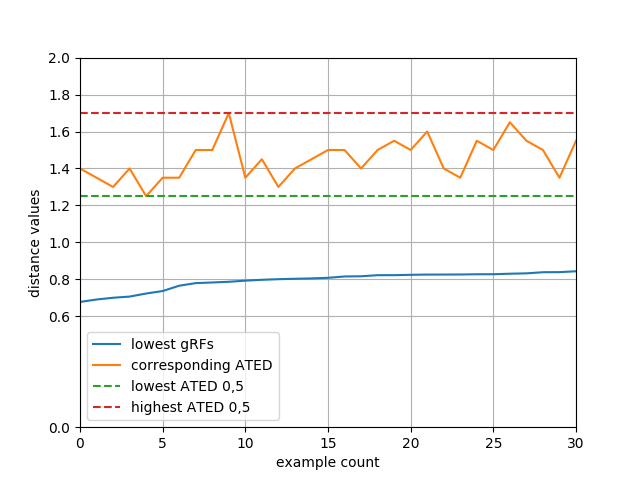
\includegraphics[width=\textwidth]{figures/low_grf_corr_ated.png}
	\end{subfigure}
	\quad
	\begin{subfigure}[b]{0.45\textwidth}
		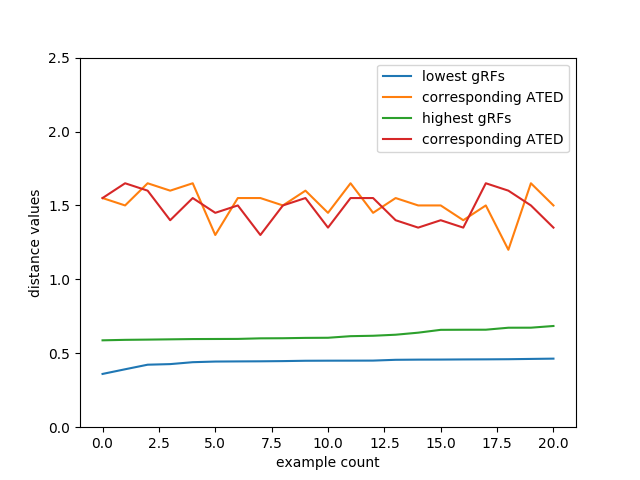
\includegraphics[width=\textwidth]{figures/high_grf_corr_ated.png}
	\end{subfigure}
	\caption{Magnifying on the extremal cases of our test instances, namely the lowest and highest $10$\% of gRF distances, gives us a good feeling about a non-existing correspondence between the gRF and the TED.}
	\label{fig:low_high_grf_corr_ated}
\end{figure} 

In Figure~\ref{fig:ex_ated_grf} we sorted the examples according to their $\frac{1}{2}$-ATED. This graph further shows, that there is no direct correlation between two trees' $\frac{1}{2}$-ATED and their gRF distance. The overall tendency is similar meaning that a higher $\frac{1}{2}$-ATED suggests a higher gRF, however the graphs show that we cannot draw any conclusions.
\begin{figure}[!ht]
	\centering	
	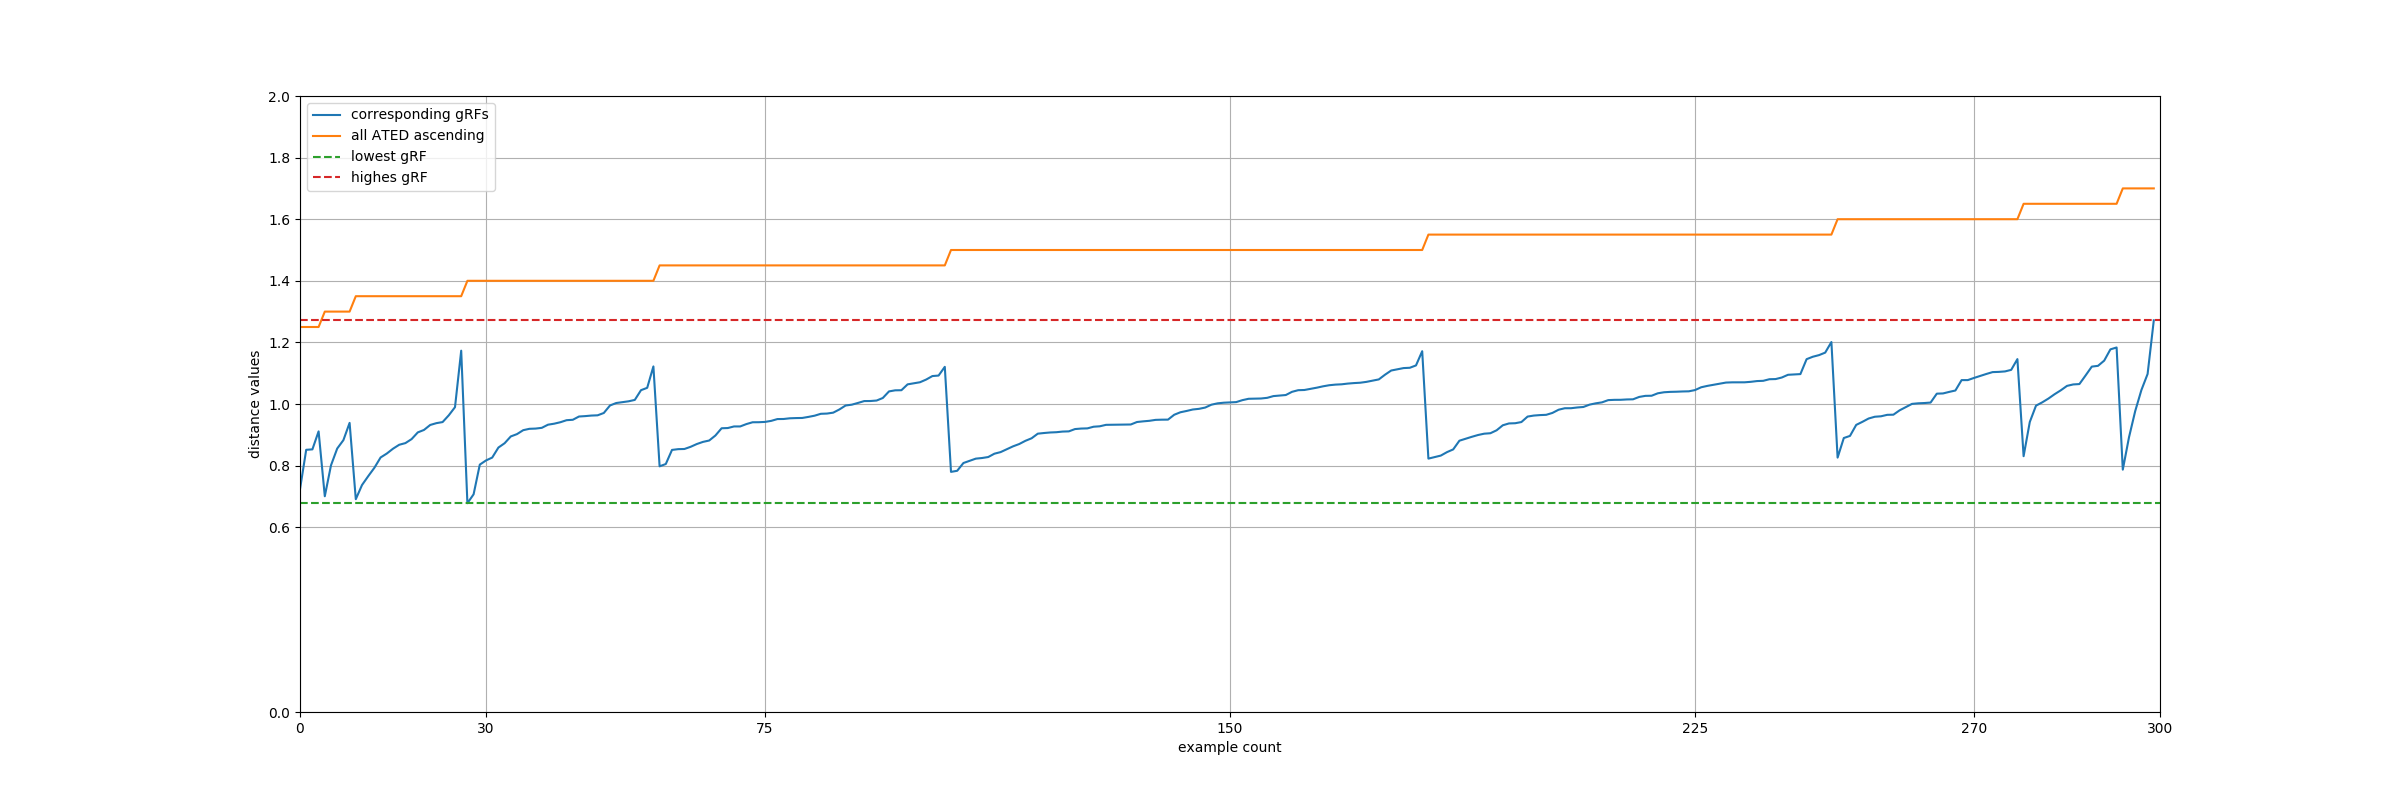
\includegraphics[width=\textwidth]{figures/all_examples_ated_corr_grf.png}
	\caption{Illustration of the distances of our randomly generated test instances, sorted increasingly with respect to the $\frac{1}{2}$-ATED distance.}
	\label{fig:ex_ated_grf}
\end{figure} 

All in all, a higher gRF suggests a higher $\frac{1}{2}$-ATED, but it is apparent, that there is no correlation between these two distance measures. Therefore it can't be possible to simulate the highly complex gRF distance with the easier $\frac{1}{2}$-ATED as our representative of TEDs.
